\documentclass[a4paper,titlepage,10pt]{article}

\usepackage[T1]{fontenc}
\usepackage[utf8]{inputenc}
\usepackage{polski}

\usepackage{enumerate}
\usepackage{amssymb}
\usepackage{amsmath}
\usepackage[pdftex]{graphicx}
\usepackage{tikz}
\usepackage[colorlinks=true,linkcolor=blue]{hyperref}
\usepackage{anysize}

\usepackage{lastpage}
\usepackage{fancyhdr}

\usepackage{pdflscape}

\usepackage[a4paper, top=2.5cm, bottom=2.5cm, left=2cm, right=2cm]{geometry}

\linespread{1.3}

\title{\huge Symulacja układu planetarnego na GPU\\ przy użyciu CUDA i OpenGL\\\small Dokumentacja końcowa\\\large Promotor: Krzysztof Kaczmarski}
\author{Daniel Kłobuszewski\and Jakub Kotur}

\begin{document}
	\maketitle
	
	\pagestyle{fancyplain}
%        \fancyhf{}
	\cfoot{\thepage/\pageref{LastPage}}

	\hfill \\
	\begin{figure}[h]
	\centering
\begin{tabular}{|p{.1\textwidth}|p{.04\textwidth}|p{.1\textwidth}|p{.1\textwidth}|p{.206\textwidth}|p{.1\textwidth}|}
	\hline
	\multicolumn{6}{|l|}{Metryka dokumentu} \\
	\hline
	Projekt & \multicolumn{2}{l|}{Symulacja układu planetarnego na GPU } &
	Firma & \multicolumn{2}{l|}{Politechnika Warszawska} \\
	&  \multicolumn{2}{l|}{przy użyciu CUDA i OpenGL} & &  \multicolumn{2}{l|}{} \\
	\hline
	Nazwa & \multicolumn{5}{l|}{Dokumentacja techniczna} \\
	\hline
	Temat & \multicolumn{5}{l|}{Specyfikacja techniczna projektu} \\
	\hline
	Autor & \multicolumn{5}{l|}{Daniel Kłobuszewski, Jakub Kotur} \\
	\hline
	Plik & \multicolumn{5}{l|}{tech.pdf} \\
	\hline
	Nr wersji & 06 & Status & Finalny & Data\par sporządzenia & 2010-10-09 \\
	\hline
	Streszczenie & \multicolumn{5}{p{11cm}|}{Celem dokumentu jest zdefiniowanie
		technicznych wymagań Projektu.} \\
	\hline
	Zatwierdził & \multicolumn{3}{l|}{ } &
	Data ostatniej\par modyfikacji & 2010-10-12 \\
	\hline
\end{tabular}

	\label{tab:metric}
\end{figure}


	\hfill \\
	%\newpage
	\begin{figure}[h]
	\centering

\begin{tabular}{|p{.075\textwidth}|p{.1\textwidth}|p{.2\textwidth}|p{.522\textwidth}|}
	\hline
	\multicolumn{4}{|l|}{Historia zmian dokumentu} \\
	\hline
	Wersja & Data & Kto & Opis \\
	\hline
	0.1 & 2011-01-02 & Jakub Kotur &
	Określenie podstawowej struktury dokumentu \\
	\hline
	0.2 & 2011-01-04 & Jakub Kotur &
	Dodanie opisów dziłania oraz zmian \\
	\hline
	1.0 & 2011-01-04 & Daniel Kłobuszewski &
	Poprawki ortograficzne i stylistyczne \\
	\hline
\end{tabular}

	\label{tab:hist}
\end{figure}



	\newpage

	\tableofcontents
	\newpage

	\section{Streszczenie}\label{sec:streszczenie}
	\paragraph{}
Poniższy dokument stanowi podsumowanie projektu, pisanego w ramach przedmiotu Projekt Zespołowy, na wydziale Matematyki i Nauk Informacyjnych Politechniki Warszawskiej w semestrze zimowym 2010/2011.

\paragraph{}
Opisujemy w nim zasady działania głównych modułów, różnice w stosunku do specyfikacji oraz wnioski z testów akceptacyjnych. Znajduje się tutaj także krótka instrukcja obsługi programu, która pozwoli zapoznać się z nim każdej osobie, która wcześniej nie miała z naszą aplikacją styczności.

	\section{Instrukcja użytkownika}\label{sec:instrukcja użytkownika}
	%\subsection{Opcje startowe}\label{sub:uruchamianie programu}
%\paragraph{}

\subsection{Poruszanie kamerą}\label{sub:poruszanie kamerą}
\paragraph{}
Kamera w aplikacji jest swobodna, co oznacza, że możemy poruszać i obracać nią we wszystkich kierunkach. Do przesuwania kamery w przód i w tył służą odpowiednio klawisze W i S. Przesunięcia w lewo i w prawo odbywają się przy pomocy klawiszy A i D, natomiast ruch w górę i w dół jest możliwy przy użyciu klawiszy Q i E. Tę ostatnią czynność możemy zrealizować także korzystając z klawisza Ctrl i spacji.
\paragraph{}
Do wykonywania obrotów należy użyć myszy. Jest ona używana także do korzystania z GUI. Do odróżnienia tych dwu czynności używany jest prawy przycisk myszy. Kiedy jest on wciśnięty, ruchy myszką odpowiadają "rozglądaniu się" w przestrzeni kosmicznej. 
\paragraph{}
Dodatkowo, jeżeli chcemy śledzić jakąś planetę, a nie chce nam się ciągle lecieć za nią kamerą, wystarczy, że klikniemy na nią lewym klawiszem myszy. Wówczas kamera automatycznie będzie zmieniała swoje położenie tak, aby nie zmieniać odległości od zaznaczonej planety. W takim trybie można dalej swobodnie się rozglądać, ale już nie poruszać. Aby wrócić do swobodnego trybu kamery, wystarczy kliknąć gdzieś w przestrzeń kosmiczną.

\subsection{Interfejs graficzny}\label{sub:interfejs graficzny}
\paragraph{}

Po uruchomieniu aplikacji pokazuje się okno przedstawiające kosmos. Na nim znajdują się również guziki. Przy ich pomocy możliwe jest wczytanie bądź zapisanie układu planet. Można również wystartować lub zatrzymać animację. Dostępne są też różne opcje programu, takie jak modyfikacji szybkości kamery, szybkości animacji oraz inne opcje graficzne i fizyczne. W tym rozdziale przedstawione będzie użycie podstawowych możliwości GUI. Dla oszczędności tuszu, kolory na obrazkach są odwrócone w porównaniu do oryginalnej aplikacji.

\begin{figure}[ht!]
\centering
\fbox{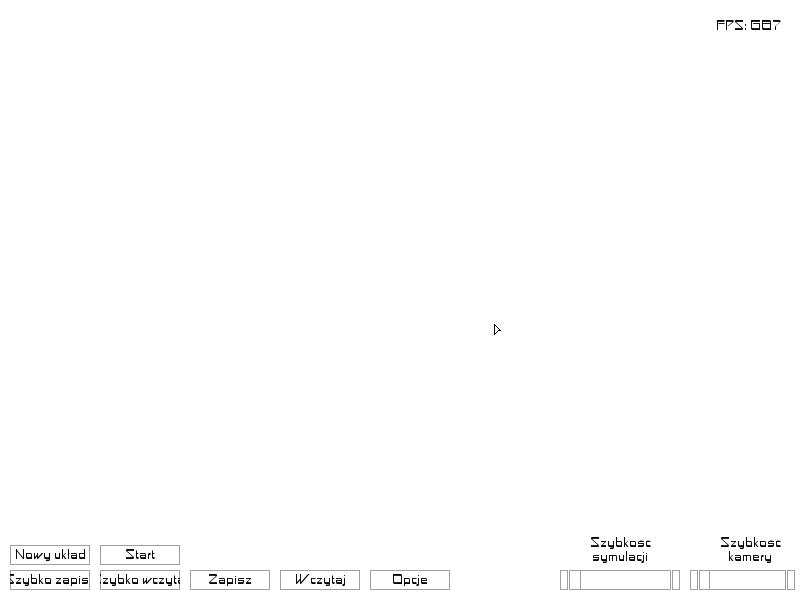
\includegraphics[width=0.75\textwidth]{img/inst_00.png}}
\caption{Początkowe okno}
\label{fig:inst_00}
\end{figure}

\subsubsection{Odczyt}\label{ssub:odczyt}
\paragraph{}

Po wciśnięciu guzika wczytaj, na ekranie pojawi się okno wczytywania. Możemy na nim wybrać interesujący nas układ. Po wybraniu układu oraz wciśnięciu "Wczytaj" układ zostanie załadowany. Można również wcisnąć guzik "Szybko wczytaj" który pozwoli na natychmiastowe wczytanie układu o nazwie "qsave.sav".

\begin{figure}[ht!]
\centering
\fbox{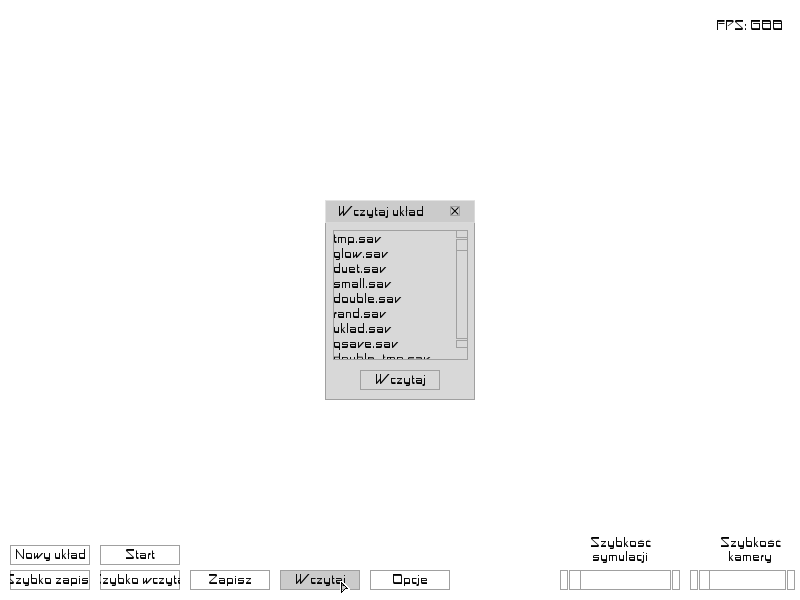
\includegraphics[width=0.75\textwidth]{img/inst_06.png}}
\caption{Okno wczytywania}
\label{fig:inst_01}
\end{figure}

\begin{figure}[ht!]
\centering
\fbox{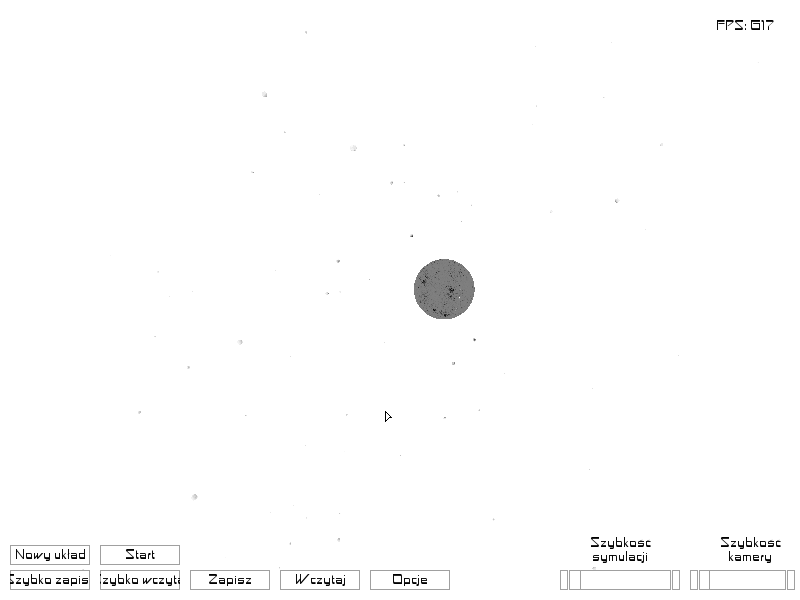
\includegraphics[width=0.75\textwidth]{img/inst_02.png}}
\caption{Wczytany układ}
\label{fig:inst_02}
\end{figure}

\subsubsection{Start animacji}\label{ssub:start animacji}
\paragraph{}

Układ domyślnie wczytywany jest w trybie pauzy. Aby wystartować animację należy wcisnąć guzik start. Powinien on w tedy zmienić nazwę i funkcję na puaza, a planety powinny zacząć się poruszać.

%\begin{figure}[ht!]
%\centering
%\fbox{\includegraphics[width=0.75\textwidth]{img/inst_03.png}}
%\caption{Animacja}
%\label{fig:inst_03}
%\end{figure}

\subsubsection{Zapis układu}\label{ssub:zapis ukladu}
\paragraph{}

Jeżeli aktualny stan układu się nam podoba, możemy go zapisać. Należy w tym celu wcisnąć guzik "Zapisz", po wciśnięciu którego na ekranie pojawi się okno. W oknie tym należy wpisać nazwę nowego układu, oraz wcisnąć guzik "Zapisz" na oknie. Od tej pory nowy układ będzie dostępny do wczytania przez aplikację.


\begin{figure}[ht!]
\centering
\fbox{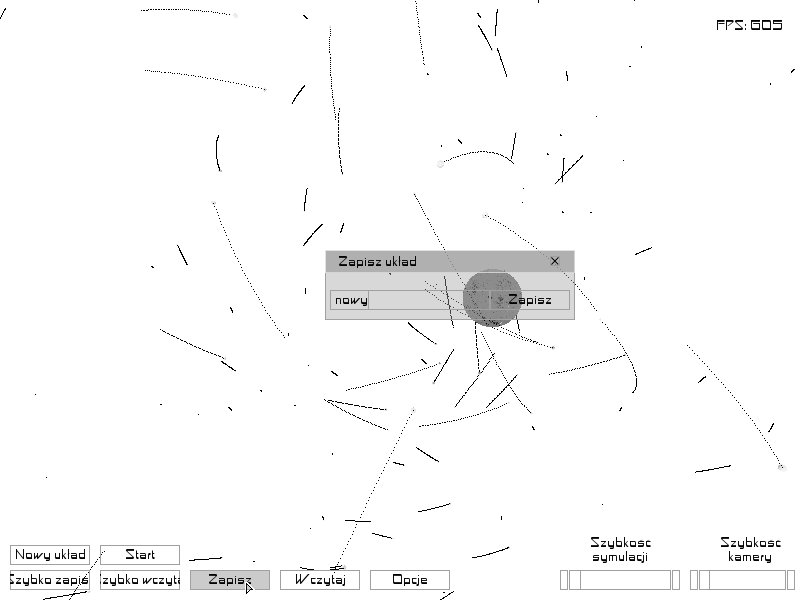
\includegraphics[width=0.75\textwidth]{img/inst_07.png}}
\caption{Okno zapisu}
\label{fig:inst_04}
\end{figure}

\subsubsection{Opcje}\label{ssub:opcje}
\paragraph{}

Na głównym ekranie znajdują się również dwa suwaki, którymi można zmieniać odpowiednio prędkość symulacji, oraz szybkość kamery. Pierwszy suwak odpowiada za liczbę klatek fizyki na jedną klatkę programu. Drugi natomiast zmienia szybkość poruszania kamery w przestrzeni. Dodatkowo po wciśnięciu guzika "Opcje" który znajduje się w głównym ekranie aplikacji, jest dostęp do dodatkowych opcji programu. Można tam manipulować ustawieniami graficznymi, fizycznymi i innymi.


	\section{Opis działania}\label{sec:opis dzialania}
	\subsection{Silnik graficzny}\label{sub:silnik graficzny}
\paragraph{}

Silnik graficzny został napisany przy użyciu techniki deferred rendering. Pozwala ona na dużą kontrolę nad procesem renderowania, oraz bardzo dobrze zachowuje się przy licznych obiektach oraz dużych przestrzeniach. W przypadku planet mamy do czynienia z takim właśnie wariantem. Dodatkowo pozwoliło to na optymalizację dzięki której geometria w programie została ograniczona do niezbędnego minimum. Powoduje to oczywiście dodatkowe koszty, jednak są one o wiele mniejsze niż w przypadku standardowego podejścia forward renderingu.

\subsubsection{Deferred rendering}\label{ssub:deferred rendering}
\paragraph{}

Deferred rendering jest ostatnio bardzo popularną techniką, używaną w wielu współczesnych grach komputerowych. Polega on na dwu przejściowym generowaniu finalnego obrazu. W pierwszym przejściu, przeliczana jest geometria, a wynik tych obliczeń wpisywany jest do specjalnego bufora ekranu. W buforze tym, znajduje się informacja o pozycji, normalnej, kolorze obiektu w danym pikselu ekranu. Mimo swoich licznych zalet, posiada on również i wady. Poniżej przedstawione są zarówno zalety, jak i wady takiego podejścia. W zależności od danego silnika bufor ten może zawierać różne dane. W drugim przejściu, na podstawie tego bufora liczone są wszystkie niezbędne efekty, takie jak oświetlenie, cienie, ambient occlusion, oraz wszelkie inne efekty graficzne. Takie podejście pozwala na bardzo wiele, oraz jest stosunkowo wydajne, posiada jednak wady. Poniżej przedstawione są wady jak i zalety deferred renderingu.

\paragraph{Zalety}

\begin{description}
\item{Skalowalność} - ponieważ wszystkie obliczenia liczone są dla piksela, silnik ten doskonale skaluje się ze względu na dodawanie geometrii do sceny
\item{Duża kontrola} - dzięki jawnemu tworzeniu buforów ekranu, można stworzyć wiele niestandardowych efektów graficznych
\end{description}

\paragraph{Wady}

\begin{description}
\item{Wielkość buforów} - bufory ekranu zajmują bardzo dużo miejsca, przy rozdzielczości full hd może być to nawet 50MB, co dla starych kart graficznych było wielkościami ogromnymi
\item{Przezroczystość} - ponieważ obliczenia są robione tylko raz dla każdego bufora, niemożliwe jest zrobienie przezroczystości w ten sposób
\item{Dużo obliczeń} - niezależnie od sceny obliczenia są proporcjonalne do wielkości ekranu i robione dla piksela. Dla starych kart graficznych jest to o wiele za ciężkie rozwiązanie
\item{Wymagane MTR} - ponieważ buforów jest wiele, wymagana od karty jest technologia MTR, czyli multiple target render, dzięki której można wygenerować za jednym zamachem wszystkie bufory. Na starych kartach graficznych potrzebne było tyle przejść ile jest buforów, co powoduje wielokrotne obliczenia geometrii
\end{description}

\subsubsection{Generowanie geometrii}\label{ssub:generowanie geometrii}
\paragraph{}

Dzięki zastosowaniu deferred renderingu, oraz tego, że renderowanymi obiektami są jedynie kule, można ominąć standardowy proces generowania geometrii. Kula która daje zadowalający efekt i jest wyświetlana przy pomocy zestawu wierzchołków, musiała by ich mieć około tysiąca. Samo przetwarzanie takiej geometrii jest kosztowne, dodatkowo doszły do tego ograniczenia karty graficznej i geometry shaderów, które trzeba by obchodzić, narażając się na dodatkowe koszty.

\paragraph{}

Wiedząc że jedyne obiekty które chcemy wyświetlić są kulami, wiemy że obiekt taki z każdej strony wygląda tak samo. Jesteśmy również w stanie łatwo policzyć składową z kuli, mając jedynie koordynaty w osiach OX i OY na tej kuli. Dzięki tym spostrzeżeniom, można stworzyć mapę głębokości (koordynat na osi OZ) kuli. Dzięki takiej mapie, w pierwszym przebiegu, wyświetlane są jedynie płaskie kwadraty, które dzięki mapie głębokości, są w stanie do bufora ekranu przekazać poprawną informację o pozycji piksela w przestrzeni. Dodatkowo ta sama mapa stanowi mapę normalnych dla oświetlenia. Dzięki takiemu podejściu, każda planeta generuje jedynie cztery wierzchołki, a reszta geometrii jest odczytywana z tekstury.

\paragraph{}

Niestety tak pięknie by to wyglądało, gdyby zastosowany był rzut ortogonalny. W symulacjach jednak konieczne do zastosowania jest rzut projekcyjny. W takim przypadku planeta widoczna na krawędzi kamery, różni się od planety widocznej na wprost. W skrajnym przypadku, gdy widoczne jest 360°, możemy widzieć planetę zupełnie od tyłu. Dlatego konieczne są dodatkowe obliczenia, uwzględniające położenie planety względem kamery.

\subsubsection{Obliczanie oświetlenia}\label{ssub:obliczanie oświetlenia}
\paragraph{}

Obliczanie oświetlenia na podstawie buforów ekranów nie stanowi problemu. W programie zastosowane jest model oświetlenia Phonga, natomiast obliczenia prowadzone są dla każdego piksela oddzielnie. Dodatkowo w celach optymalizacyjnych, nie jest liczone światło odbite (specular), ponieważ planety mają powierzchnię chropowatą, więc i tak oświetlenie to by miało znikomy wpływ na efekt końcowy, natomiast jest dość kosztowne obliczeniowo.

\paragraph{}

W celu optymalizacji, dodatkowo do każdej gwiazdy (źródła światła) przypisany jest jej zakres świecenia. Dzięki temu oświetlenie z gwiazd, które nie oświetlają planet odległych od siebie, nie jest obliczane. W przypadku gwiazd nie jest to tak znaczna optymalizacja jak w przypadku bardzo słabych świateł, jak na przykład lampki choinkowe, jednak sprawdza się przy kilku odległych od siebie galaktykach.

\subsubsection{Nakładanie tekstur}\label{ssub:nakladanie tekstur}
\paragraph{}

Skomplikowaniu ze względu na użycie deferred renderingu uległo niestety nakładanie tekstur na planety. Tekstura, tak samo jak wspomniana wcześniej mapa normalnych, jest nakładana na kulę w zależności od koordynat na osiach OX i OY. Jednak w odróżnieniu od mapy normalnych, tekstura zależy od obrotu kamery względem planety, i z każdej strony wygląda inaczej. Pojawiły się więc dwa problemy. Obracanie koordynat tekstury, tak aby widz miał wrażenie że planeta faktycznie się obraca, oraz mapowanie koordynat kwadratu reprezentującego planetę, na koordynaty tekstury planety.

\paragraph{}

Pierwszy problem został rozwiązany poprzez przekazywanie obrotu kamery do silnika graficznego, poprzez przekazanie macierzy obrotu kamery. Następnie uzyskane koordynaty kuli, są przemnażane przez tą macierz. W ten sposób otrzymywany jest bezwzględna pozycja kuli, na którą patrzy aktualnie kamera.

\paragraph{}

Drugim problemem jest mapowanie tekstury na kulę, tak aby z koordynat kuli 3D, uzyskać koordynaty na teksturze 2D. W standardowym podejściu, stosuje się siatki tekstury, natomiast każdy trójkąt jest interpolowany na płaszczyźnie. W naszym podejściu nie ma trójkątów, trzeba więc było uzyskać ciągły sposób mapowania, bez żadnych siatek. Z pomocą przyszła kartografia, która zna liczne sposoby mapowania płaszczyzny na kulę i z powrotem. Najlepsze okazały się metody mapowania o stałej powierzchni. Oznacza to że parametrem który nie ulega zniekształceniu ze względu na położenie na kuli, jest powierzchnia. Dzięki temu po mapowaniu tekstury na kulę, zniekształcenia są najmniejsze. Najtańszą obliczeniowo z tych metod okazała się metoda sinusoidalna, która wymaga policzenia jedynie jednego sinusa.

%\subsubsection{Atmosfery}\label{ssub:atmosfery}
%\paragraph{}

\subsection{Silnik fizyczny}

\subsubsection{Klastertyzacja}

\paragraph{} Do klasteryzacji używany jest alorytm k-means. Klastry definiowane są przez dwie tablice - \ensuremath{shuffle} oraz \ensuremath{count}. Do klastra o numerze k należą te planety, których indeksy znajdują się w tablicy \ensuremath{shuffle} pod indeksami z przedziału \ensuremath{< count[k-1], count[k] )}. Przyjmujemy, że \ensuremath{count[-1] = 0}.

\paragraph{} Taka reprezentacja pozwala na łatwe korzystanie z planet z danego klastra w module fizycznym i jest transparentna dla modułu graficznego.

\subsubsection{Kolizje} w teorii rozwiązywane są prosto - jeżeli dwa obiekty zachodzą na siebie, należy je skleić. Algorytm sekwencyjny do tego celu sprawdzałby kolejne pary planet, usuwając te kolidujące ze sobą. Jeżeli jednak chcemy zrealizować obsługę kolizji równolegle, rozwiązanie naiwne okazuje się nie być prawidłowe. Gdyby każda planeta w osobnym wątku CUDA sprawdzała kolizje ze wszystkimi planetami po kolei, mogłoby dojść do konfliktów.

\paragraph{} Najpierw opiszę sposób, w jaki usuwamy planety. Przy każdej kolizji jedna planeta musi zostać usunięta, a druga staje się sumą fizyczną tych dwóch planet. Usuwanie planet przebiega dwuetapowo. Pierwszy etap, usunięcie logiczne, to zwykłe wyzerowanie masy oraz promienia usuwanej planety. Wyzerowanie masy powoduje, że planeta nie oddziałuje na inne, jest więc transparentna dla modułu fizyki. Wyzerowanie promienia natomiast "ukrywa" planetę przed modułem graficznym, który dzięki temu jej nie wyświetla. Dodatkowo, algorytm wykrywający kolizje ignoruje planety o zerowym promieniu.
Drugi etap usuwania, usunięcie fizyczne, powoduje przesunięcie wszystkich "istniejących" planet do początku tablicy - dla każdego parametru osobno. Realizowane jest to przy pomocy funkcji cudppCompact z biblioteki cudpp.
Wewnątrz tej funkcji, używana jest funkcja cudppScan, która efektywnie zamienia tablicę zerojedynkową, odróżniającą planety nieusunięte od usuniętych, na tablicę indeksów, pod które należy skopiować te planety.

\paragraph{} Wracając do problemu z równoległością w rozwiązywaniu kolizji - w implementacji naiwnej mogłoby się zdarzyć tak, że dwie planety w tym samym czasie wykryłyby kolizję z trzecią planetą, obliczyłyby parametry wynikowej planety (każda ze sobą), po czym wyzerowałyby parametry tej planety. W efekcie kolidująca planeta zostałaby "zdublowana" - w szczególności jej masa dodałaby się do obu kolidujących z nią planet.

\paragraph{} Obsługa kolizji przebiega w efekcie dwuetapowo: pierwszy etap to wykrycie kolizji, drugi to ich rozwiązanie, czyli sklejanie kolidujących planet. Poza wymienionymi wyżej czynnikami należy wspomnieć o jeszcze jednym - o klasteryzacji. Kolizje rozwiązywane są jedynie wewnątrz klastrów, gdyż zakładamy, że prawdopodobieństwo kolizji planet z różnych klastrów jest pomijalnie niewielkie.

\paragraph{Detekcja kolizji} - definiujemy tablicę kolizji k. Jeżeli planeta i nie koliduje z żadną, \ensuremath{k[i] = i}. Jeżeli natomiast wykryła kolizję z planetą j, \ensuremath{k[i] = j}. Dodatkowo wymagamy, żeby relacja ta spełniała warunek \ensuremath{i\prec j} w pewnym porządku liniowym. Dzięki temu kolidujące planety nie utworzą cyklu.

\paragraph{} Kolizje rozwiązujemy wewnątrz klastra.  Z definicji tablicy shuffle wynika, że \ensuremath{i \neq j \Rightarrow shuffle[i]\neq shuffle[j]}. Wobec tego relacja \ensuremath{shuffle[i] \prec shuffle[j] \Leftrightarrow i<j } tworzy porządek liniowy.

\paragraph{} Detekcja przebiega następująco:
\begin{lstlisting}
merge_needed = false
foreach planet p in parallel
	id = p.index + 1
	while id < count[ p.cluster ]
		if( kolizja( p, planet[ shuffle[ id ] ] ) )
			merge_needed = true
			k[ shuffle[ p.id ] ] = shuffle[ id ]
			return;
		++id
	k[ shuffle[ p.id ] ] = shuffle[ p.id ]
\end{lstlisting}

\paragraph{} W efekcie dostajemy tablicę k. Jeżeli nie została ustawiona flaga merge\_needed, kończymy. Jeżeli została, zaczynamy sklejanie planet:
\begin{lstlisting}
done = false
k_in = k
while !done
	done = true
	foreach planet p in parallel	
		if( k_in[ p.id ] == p.id )
			k_out[ p.id ] = p.id
			return
		if( k_in[ k_in[ p.id ] ] != k_in[ p.id ] )
			k_out[ p.id ] = k_in[ p.id ]
			done = false
		merge( p, planet[ k_in[ p.id ] ] )
		k_out[ p.id ] = p.id
	k_in <=> k_out
\end{lstlisting}

\paragraph{} Po czym powtarzamy detekcję.

	\section{Dokumentacja}\label{sec:dokumentacja}
	\paragraph{}

Dokumentacja została wygenerowana za pomocą programu Doxygen z komentarzy tworzonych podczas pisania kodu. Może być ona dostępna zarówno jako strona html oraz jako dokument w formacie pdf. Jednak z powodu dużych rozmiarów wygenerowanego dokumentu zdecydowaliśmy się na pozostawienie go w formie elektronicznej.


	\section{Raport z testów}\label{sec:raport z testów}
	\subsection{Silnik graficzny}\label{sub:silnik graficzny}

\subsection{Silnik fizyczny}\label{sub:silnik fizyczny}


	\section{Opis zmian}\label{sec:opis zmian}
	\subsection{Silnik graficzny}\label{sub:silnik graficzny}
\subsubsection{Geometria}\label{ssub:geometria}
\paragraph{}

Największą zmianą dla silnika graficznego była zmiana podejścia renderowania planet. W pierwotnych założeniach użyty miał zostać standardowy forward rendering, który wymaga siatek zarówno dla geometrii, jak i do tekstur. Po testach, okazało się że z powodów ograniczeń technicznych zastosowanie forward renderingu w takiej formie w jakiej chcieliśmy jest niemożliwe. Przeszkodą były ograniczenia karty graficznej, która pozwala na generowanie zaledwie około 100 wierzchołków przy pomocy geometry shaderów. Dla realistycznego wyglądu kuli potrzebne było natomiast przy zbliżeniach około 1000. Wszelkie podejścia wyświetlenia tak dużej geometrii prosto z karty graficznej, były skazane na niepowodzenie. Dlatego zdecydowaliśmy się na użycie techniki nazywanej deferred renderingiem. Ma ona te zalety że skaluje się bardzo dobrze dla wielu obiektów, oraz można było przy jej pomocy uzyskać realistyczne kule bez dużej ilości geometrii w programie. Wadami takiego rozwiązania są dość duże koszty, związane ze sporymi buforami ekranu, oraz obliczeniami per-piksel. Dodatkowo na starszych kartach bez MTR (Multiple Render Targets), są dodatkowe nakłady związane z wymuszonym robieniem kilku przejść. W efekcie silnik graficzny, aby działać wydajnie potrzebuje dość nowych kart graficznych, co i tak było wymuszone przez użycie CUDA w silniku fizycznym.

\paragraph{}

Powiązana zmiana z wyżej wymienioną dotyczy dynamicznego generowania geometrii. W pierwotnych założeniach siatki planet miały być generowane na różnym poziomie dokładności, następnie wyświetlana miała być właściwa dla danej planety. W podejściu deferred renderingu nie jest to konieczne, ponieważ obliczenia są robione dla każdego piksela. Oznacza to, że jeśli planeta widoczna jest jako kilka pikseli, obliczenia dla niej będą wykonywane tylko dla tych kilku pikseli. Deferred rendering w tym przypadku skaluje się idealnie, i nie ma potrzeby poprawiania go.

\subsubsection{Pamięć}\label{ssub:pamiec}
\paragraph{}

Użycie deferred renderingu poniosło za sobą pewne zmiany w strukturze programu. Niepotrzebne okazały się wszelkie struktury odpowiedzialne za generowanie, oraz przetrzymywanie geometrii. Konieczne natomiast stało się generowanie map normalnych, oraz map atmosfery. Jednak to zadanie silnik graficzny realizuje sam, dlatego w efekcie zarządzanie pamięcią się uprościło, na rzecz skomplikowania silnika graficznego.

\subsubsection{Struktura programu}\label{ssub:struktura programu}
\paragraph{}

Podejście deferred renderingu spowodowało również to, że silnik graficzny musi mieć wszystko pod swoją kontrolą. Nie można już założyć że każdy efekt graficzny komunikuje się niezależnie z openglem. Spowodowane jest to niestandardowym podejściem do wyświetlania planet. Dlatego usunięte z struktury programu zostały oddzielne klasy realizujące każdy efekt graficzny, na rzecz jednej klasy wyświetlającej całość planet.

\subsubsection{Klikanie}\label{ssub:klikanie}
\paragraph{}

Niestandardowy silnik graficzny spowodował również, że niemożliwe było użycie bezpośrednio opengla do sprawdzania która planeta została kliknięta. Konieczne było napisanie swojego rozwiązania. Bazuje ono mocno na podejściu które można znaleźć w openglu, jednak jest napisane ręcznie.

\subsection{Silnik fizyczny}\label{sub:silnik fizyczny}
\subsubsection{Kolizje}
\paragraph{}

Z powodu braku dobrego modelu fizycznego jedynym wynikiem kolizji jest w tej chwili sklejenie dwóch planet w jedną. Wynik takiego sklejenia ma masę równą sumie mas planet przed zderzeniem, objętość równą sumie objętości, oraz pęd równy sumie pędów - czyli wypadkowa prędkość powstałego tworu jest równa średniej ważonej prędkości zderzających się planet, z wagami równymi masom.

Zależność tę widać poniżej:
\begin{align}
p_3 & = p_1 + p_2 \\
m_3 * V_3 & = m_1 * V_1 + m_2 * V_2 \\
( m_1 + m_2 ) * V_3 & = m_1 * V_1 + m_2 * V_2 \\
V_3 & = \frac{ m_1 * V_1 + m_2 * V_2 }{ m_1 + m_2 }
\end{align}

\subsubsection{Organizacja kodu}

\paragraph{}

Główną zmianą w module fizycznym w stosunku do dokumentacji technicznej jest brak wspólnego interfejsu CudaAlgorithm. Pojawiła się natomiast klasa Clusterer, dzieląca przestrzeń na klastry. Konieczność jej wydzielenia wynikała ze złożoności kodu implementującego algorytm k-means.

Pewną zmianą jest także rezygnacja z przestrzeni nazw CPU2GPU oraz FILE2CPU. Zmieniona została również nazwa Holder na PlanetHolder - jako kontener służący do przechowywania informacji o planetach. Stało się tak dla odróżnienia go od ClusterHoldera przechowującego bufory z informacjami o klastrach.





\end{document}

